\chapter{Introduction and theory overview}

\section{Introduction}
This thesis presents the result and process of the search for signal of heavy resonances decaying into a Z boson and a Higgs boson (h) final state at center-of-mass energy of 8 TeV, using 19.7 $fb^{-1}$ p-p collision data. In turn, the Z boson is identified through its leptonic decays (leptons often refer to $e$ and $\mu$ only in experiments, $l = e, \mu$). The Higgs boson h is expected to hadronically decay primarily into a pair of b-quarks. The investigated final states consists of two b-quarks and two charged leptons.



\section{Theory overview}
The standard model (SM) is a great theory that has successfully explained the interaction between particles and agree with the result from experiments pretty well for past 40 
years. However, there are still serveral fundamental questions not explained in SM. One of them is mass hierarchy of quarks and leptons. 
\newline A possible solution is to introduce the compositness model \cite{preons-idea, compositeness, eichten}.  
In compositness model, quarks and leptons are claimed to be the bound states of some sub-particles. These sub-particles, called preons,  
are proposed to be bounded by an unknown interaction. The appearance of preons' idea is not surprised. In the past, various atoms are considered to be the basic unit of nature. After people break into the atoms, 
they are found to be composed of electrons, protons, and neutrons. Today, protons and neutrons are again known to be compositness. It's very intuitive to guess that the SM particles are again composed of some more fundamental 
structure. If the sub-structure of leptons or quarks really exsist, the discovery of the excited state can provide a direct proof for compositness model.  

\subsection{Model of excited leptons}
Unlike the search of Higgs boson or other theory such as supersymmetry, compositeness model is not predicted by SM and does not build up a beautiful and giant model. Furthermore, it also unlike the dark matter, which is 
suggested to be exsisted by cosmos observation. Despite there has yet a complete model of preons that can satisfies a number of physicists, the search of excited leptons has been performed at
LEP, HERA, Tevatron and the LHC before\cite{tevatron1, tevatron2, tevatron3, tevatron4, EXO-10-016, an-11-452, an-12-013, atlas2011-limit}. The behavior of the excited leptons in this thesis is simulated 
by PYTHIA 8\cite{Sjostrand:2006za}, and it uses the phenomenology described in \cite{compositeness}. 
\newline
The weak isodoublets of both left- and right-handed excited lepton of first generation are assigned as follows.

\begin{center}
$l^{*}_{L} = e_{R}\left(
\begin{aligned}
~\nu^{*}_{e}~ \\
~e^{*}~
\end{aligned}
\right)_{L}
 ~,~ 
l^{*}_{R} = \left(
\begin{aligned}
~\nu^{*}_{e}~ \\
~e^{*}~
\end{aligned}
\right)_{R}
 $
\end{center}   
It is expected that the excited leptons acquire the mass before $SU(2)\times U(1)$ symmetry breaking. The quantum numbers of excited leptons are fixed to the numbers list in Tab. \ref{tab:qn}.
Both the spin and weak isospin is set to 1/2, and hypercharge Y is set to -1.

\begin{table}[h!]
 \renewcommand{\arraystretch}{2}
 \addtolength{\tabcolsep}{5pt}
\begin{center}
\begin{tabular}{lcccc}
\hline 
\hline
 & $Y$ & $T$ & $T_{3}$ & $Q$ \\ 
\hline
$\nu_{e L}^{*}$ & -1 & $\frac{1}{2}$ & $\frac{1}{2}$ & 0 \\ 
$e^{*}_{L}$ & -1 & $\frac{1}{2}$ & $-\frac{1}{2}$ & -1 \\ 
$\nu_{e R}^{*}$ & -1 & $\frac{1}{2}$ & $\frac{1}{2}$ & 0 \\ 
$e^{*}_{R}$ & -1 & $\frac{1}{2}$ & $-\frac{1}{2}$ & -1 \\ 
\hline
\hline
\end{tabular}
\end{center}
\caption{\label{tab:qn}Quantum numbers of excited leptons.}
\end{table}

The coupling of excited leptons is assumed to have a similar form as their SM ground state. Following Lagrangian shows the interaction between two excited leptons mediate by gauge boson.
\begin{align}
 \mathcal{L}_{l^{*}l^{*}V} = \bar{l}^{*}\gamma^{\mu}\left\lgroup  g\frac{\tau}{2}W_{\mu} + g^{\prime}\frac{Y}{2}B_{\mu} \right\rgroup l^{*}
\end{align}
\noindent Due to the composite nature of the model, each interaction above should be corrected by a set of form factors. However, for a large value of the compositness scale $\Lambda$, the effect of form factors are negligible.

Gauge bosons can also mediate the transitions between right-handed excited leptons and left-handed SM leptons. This interaction leaves a signature to discover excited lepton by searching for resonance of SM leptons. The Lagrangian of excited leptons transition is written as below

\begin{align}
\mathcal{L}_{l^{*}lV} = \frac{1}{2\Lambda}\bar{l}_{R}^{*}\sigma^{\mu\nu} \left\lgroup gf\frac{\tau}{2}W_{\mu\nu} + g^{\prime}f^{\prime}\frac{Y}{2}B_{\mu\nu} \right\rgroup l_{L} + h.c.
\end{align}  

\noindent In this Lagrngian, there are two constant parameters $f$ and $f^{\prime}$, which determines the coupleing strength of different gauge fields. These two parameters are both expected to be of order 1. In this study, the final limits of excited electrons and muons are presented under the condition assuming $f = f^{\prime} = 1$ and $f = -f^{\prime} = -1$. 
 
The excited leptons may couples to SM lepton via four-fermion contact interaction source by an unknown interaction beyond SM. For energies below compositness scale $\Lambda$, they can be described by an following Lagrangian.

\begin{align}
\mathcal{L}_{CI} = \frac{g^{*2}}{2\Lambda^{2}}j^{\mu}j_{\mu}
\end{align}

\noindent The $g^{*2}$ here is chosen to have value 4$\pi$. $j^{\mu}$ is the lepton current with the form

\begin{align}
j_{\mu} = \eta_{L}\bar{f}_{L}\gamma_{\mu}f_{L} + \eta_{L}^{\prime}\bar{f}_{L}^{*}\gamma_{\mu}f_{L}^{*} + \eta_{L}^{\prime\prime}\bar{f}_{L}^{*}\gamma_{\mu}f_{L} + h.c. + (L \rightarrow R)
\end{align}

\noindent The $\eta$ factors of left-handed currents are set to be one for simplicity, and the right-handed terms are therefore become zero to reserve chiral symmetry\cite{Norm}. The $f$ and $f^{*}$ show in above equation represent fermion and excited fermion respectively. The use of ``fermion'' instead of ``lepton'' in the contact interaction Lagrangian is because of the production of excited leptons in LHC require to include the coupling of excited leptons and quarks. Leptons and quarks are assumed to be composed of same set of preons in current model, thus it is possible to have such a four-fermion contact interaction that directly couples quarks to leptons with any combination between excited and SM particles.
\newline Fig. \ref{fig:ExLep_vtxs} summarize the vertices introduced in above three Lagrangians. The intrested process of the search with four-lepton final state in CMS is shown in Fig. \ref{fig:Feyman_ExLep}. Excited leptons in this search are produced by contact interaction with a SM partner with same flavor, and transit to SM lepton via Z emission. Futhermore, the emitted Z with electron or muon decay is chosen for it provide a clean signature. The choice of Z-mediated channel is due to the relative less background events compares to $\gamma$-mediated channel, and is never been tried in LHC before, though the cross section is relative smaller. The reason of the pair production, which produced two excited leptons in one collision, is not considered in this search is that the cross section of the pair production is much smaller than the single production and can hardly raise the event yields. More details about production rate will be introduced in Sec. \ref{sec:production}.
%According to the Lagrangian, an excited lepton is allowed to transit to a SM lepton via an electroweak process. This analysis presents the search for excited leptons with 
%4-leptons in the final state. Fig. \ref{fig:Feyman_mu} and Fig. \ref{fig:Feyman_e} show the interested decay processes of $\mu^{*}$ and $e^{*}$ respectively. The data is collected 
%by the Compact Muon Solenoid (CMS) detector~\cite{cms, ptdr1, ptdr2} at the LHC with proton-proton collision at a center-of-mass energy  
%of 8 TeV. The integrated luminosity corresponds to 19.7 $fb^{-1}$ \cite{lumi001}. Searching for excited leptons in the $\ell\ell\gamma$ final state have been performed at 
%LEP, HERA, Tevatron and the LHC before, but found no evidence \cite{tevatron1, tevatron2, tevatron3, tevatron4, EXO-10-016, an-11-452, an-12-013, atlas2011-limit}. 
%This is the first attempt to search for the footprint of excited leptons in the 4-lepton channel, where a Z is radiated instead of a photon.  Although the branching ratio of 
%Z-mediated processes, shown in Fig. \ref{fig:BR_ExLep}, is much smaller than the $\gamma$-mediated process, the 4-lepton final state gives less background than $\ell\ell\gamma$. 
%The SM ZZ production is the dominating and largely irreducible background in the 4-lepton analysis. Therefore, the background estimation is fully be done by Monte-Carlo for 
%convenience.    
\begin{figure}
    \centering
    \subfigure[]
    {
        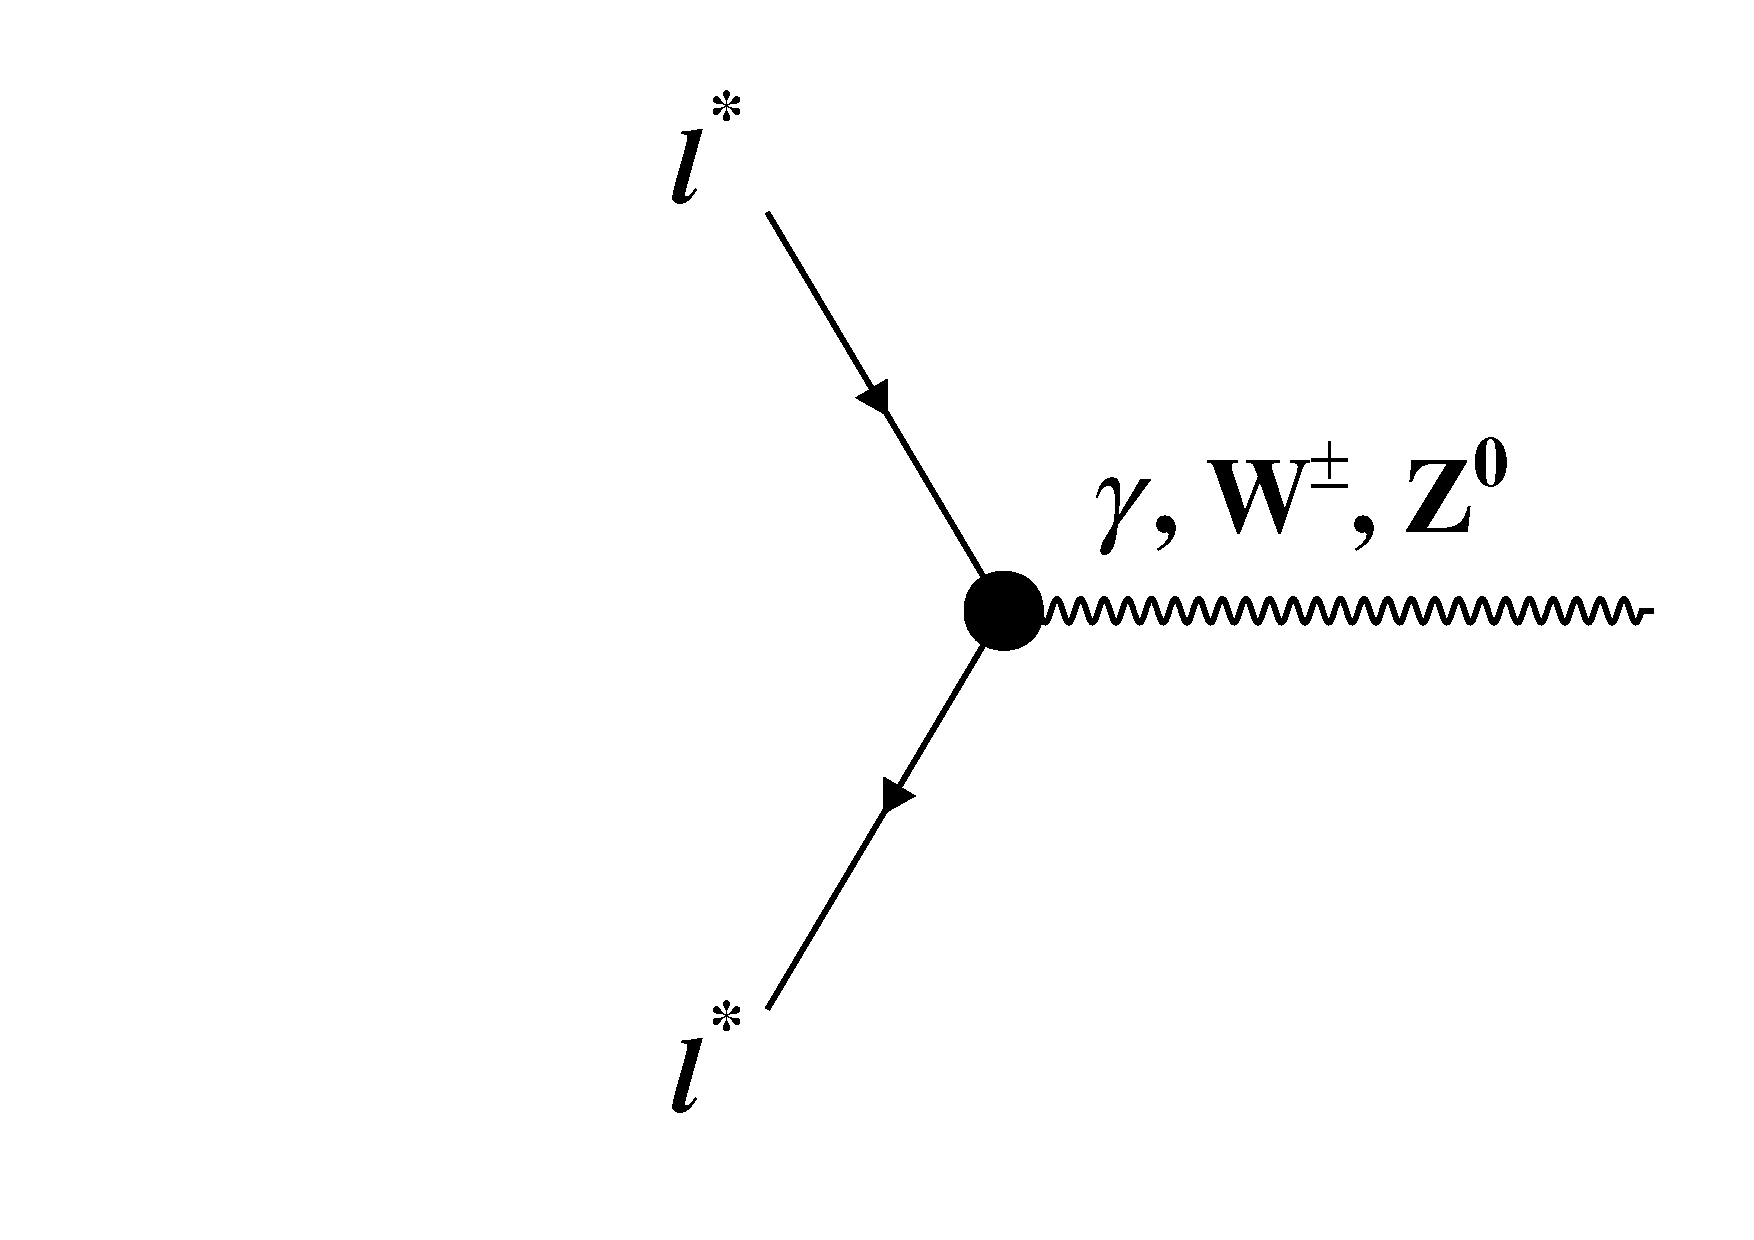
\includegraphics[width=0.35\textwidth]{plot/pair.pdf}
        \label{fig:ExLep_Gp}
    }
    \\
    \subfigure[]
    {
        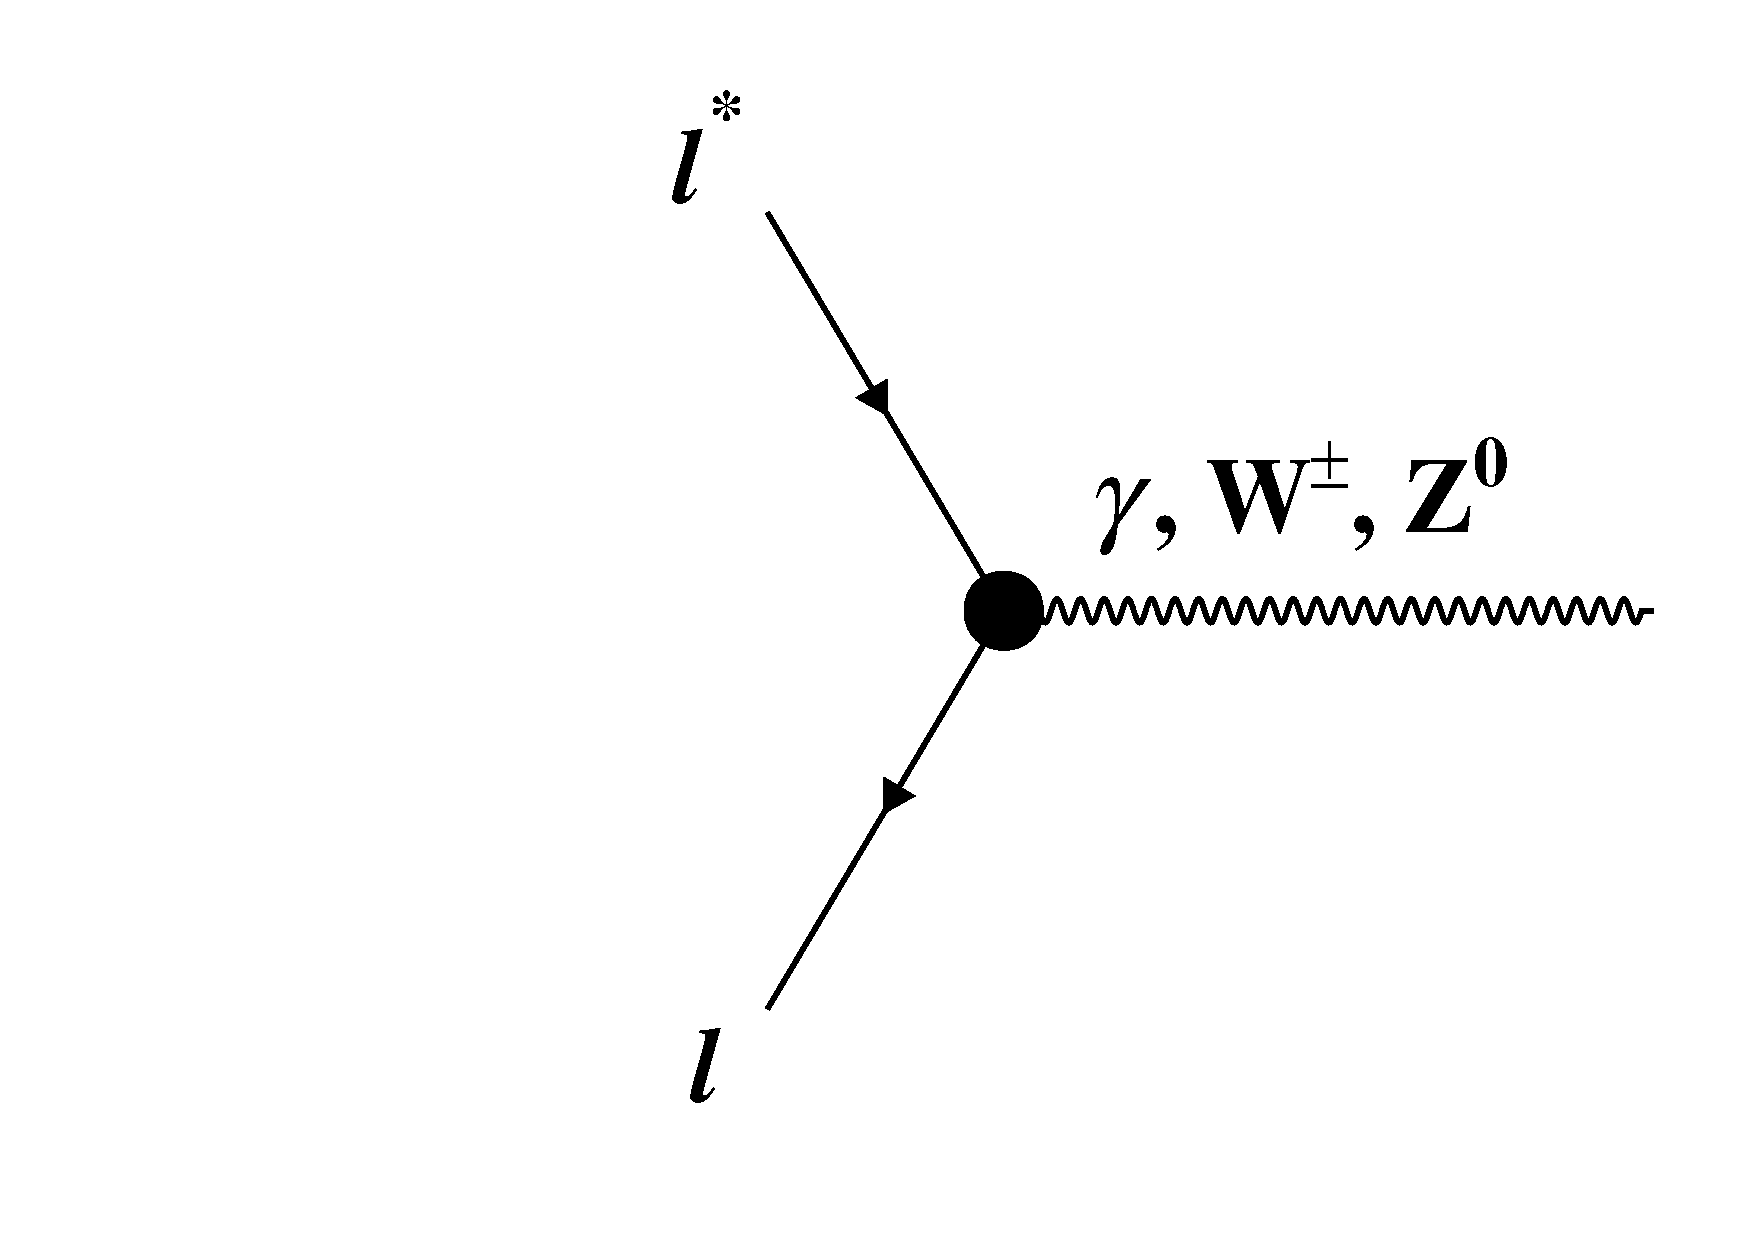
\includegraphics[width=0.35\textwidth]{plot/single.pdf}
        \label{fig:ExLep_Gs}
    }
    \\
    \subfigure[]
    {
        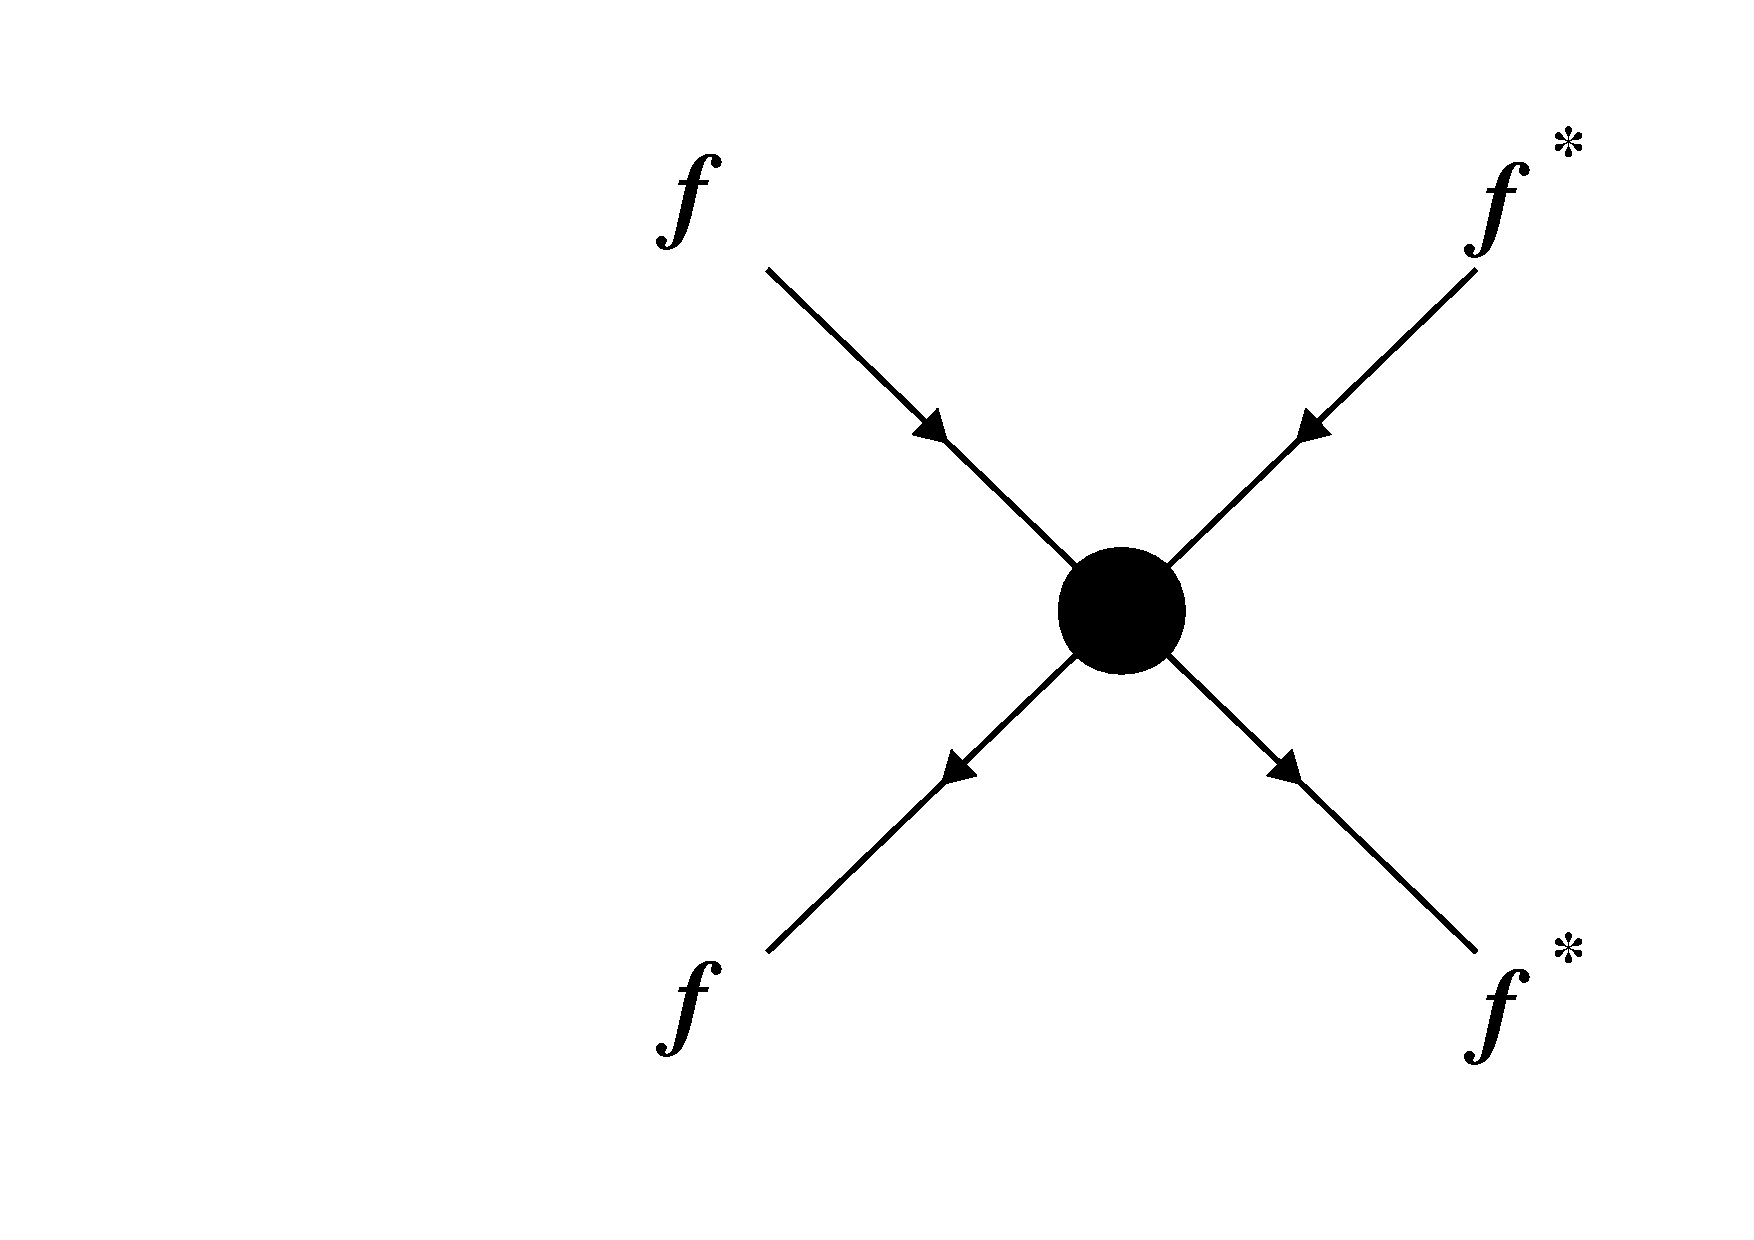
\includegraphics[width=0.35\textwidth]{plot/CIp.pdf}
        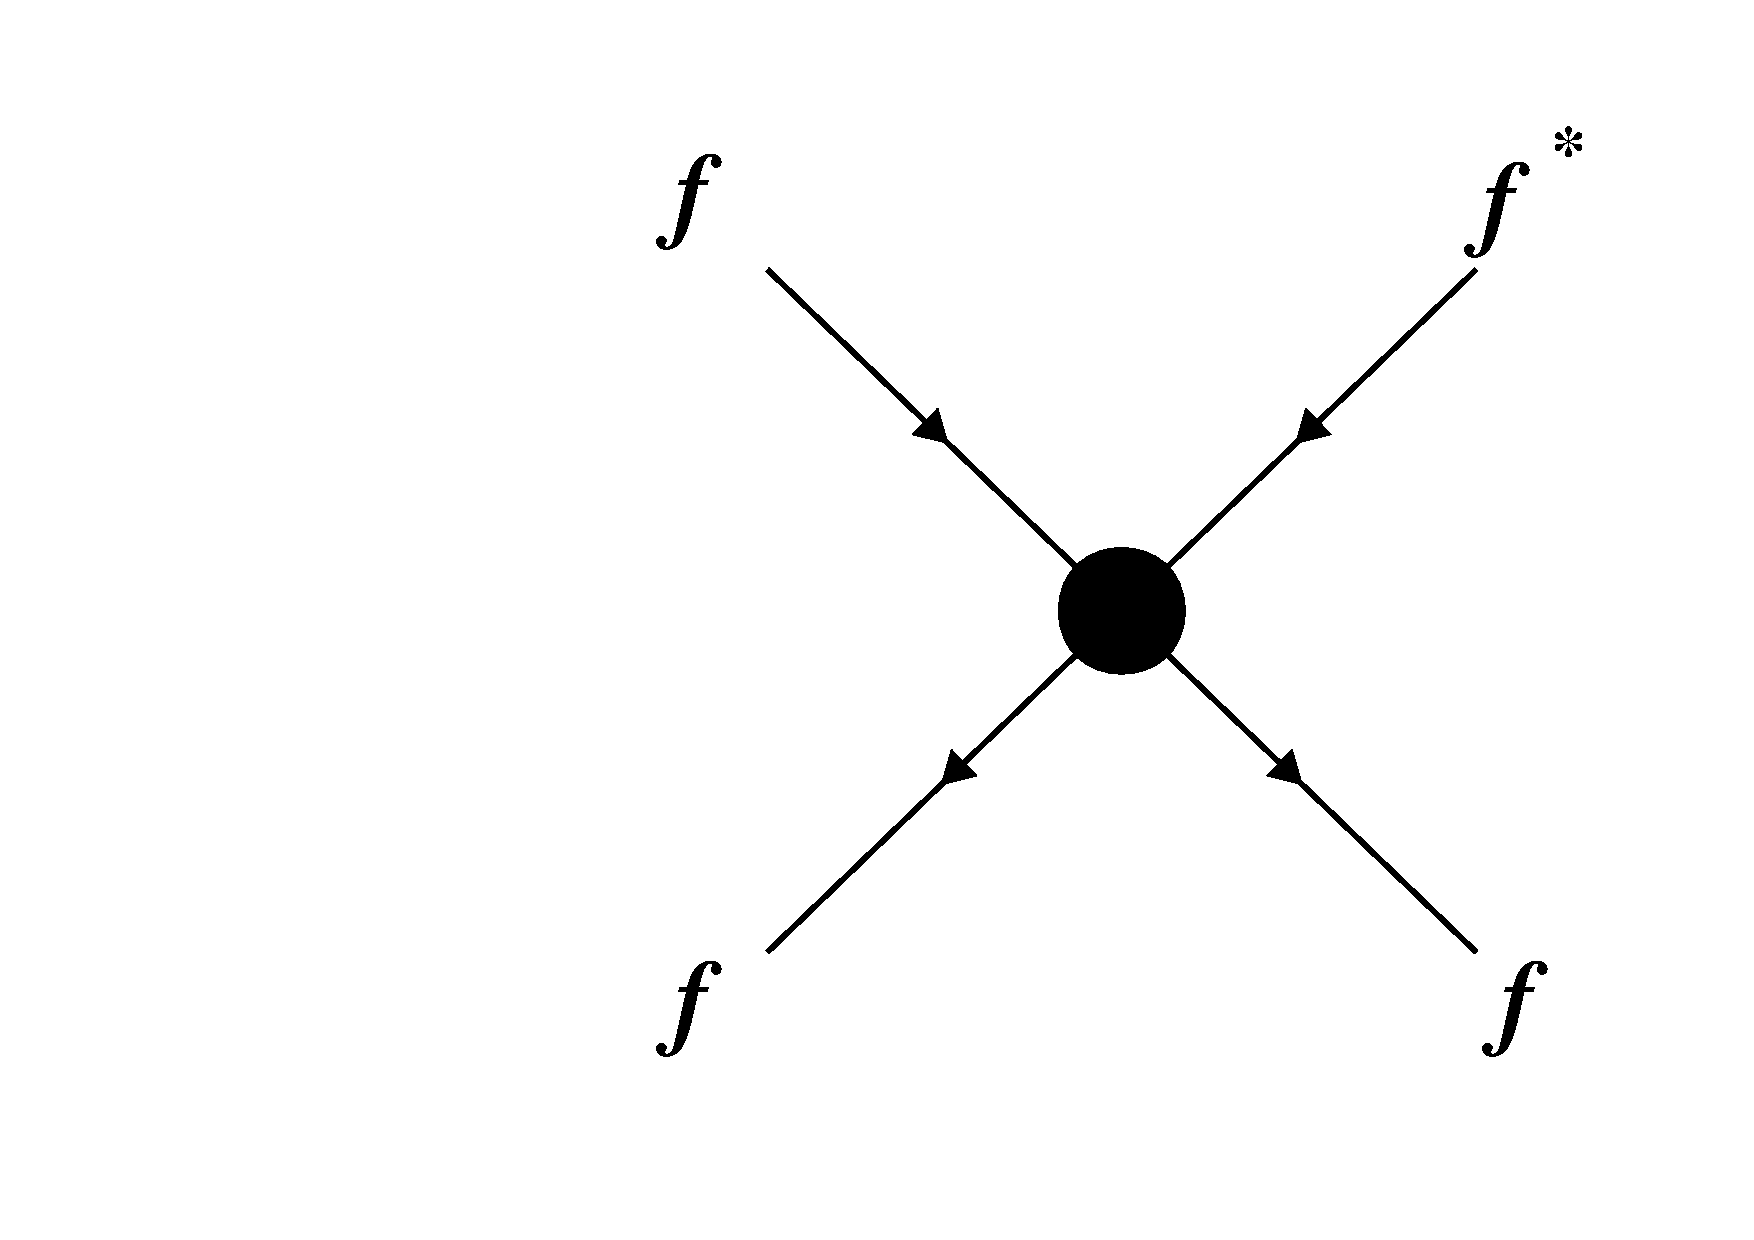
\includegraphics[width=0.35\textwidth]{plot/CIs.pdf}        
        \label{fig:ExLep_CI}
    }
    \caption{Diagrams showing excited leptons interaction vertices. (a) Gauge interaction between two excited leptons. (b) Gauge interaction between excited lepton and standard model lepton. (c) Four-fermion contact interaction.}
    \label{fig:ExLep_vtxs}
\end{figure}

\begin{figure}[h!]
\centering
\subfigure[]{
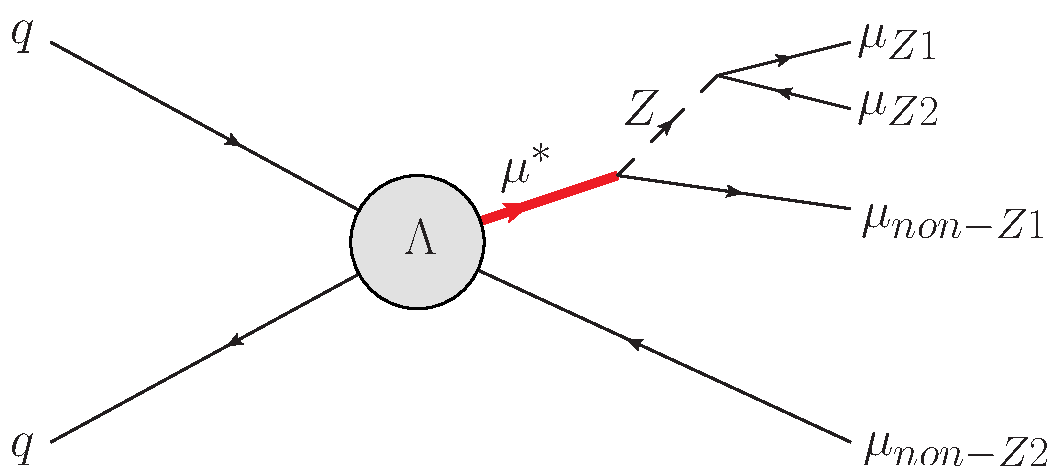
\includegraphics[width=0.49\textwidth]{plot/Feynman_Mustar4mu.pdf}
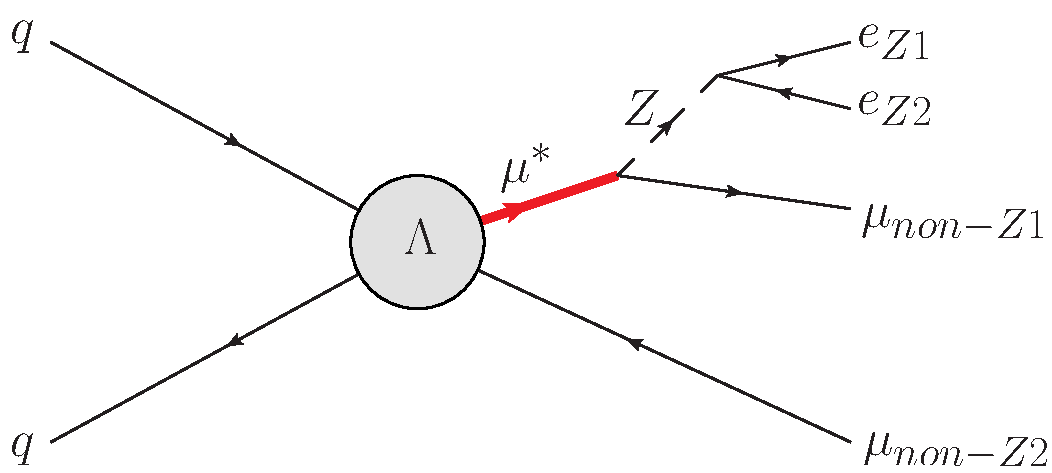
\includegraphics[width=0.49\textwidth]{plot/Feynman_Mustar2mu2e.pdf}
}
\\
\subfigure[]{
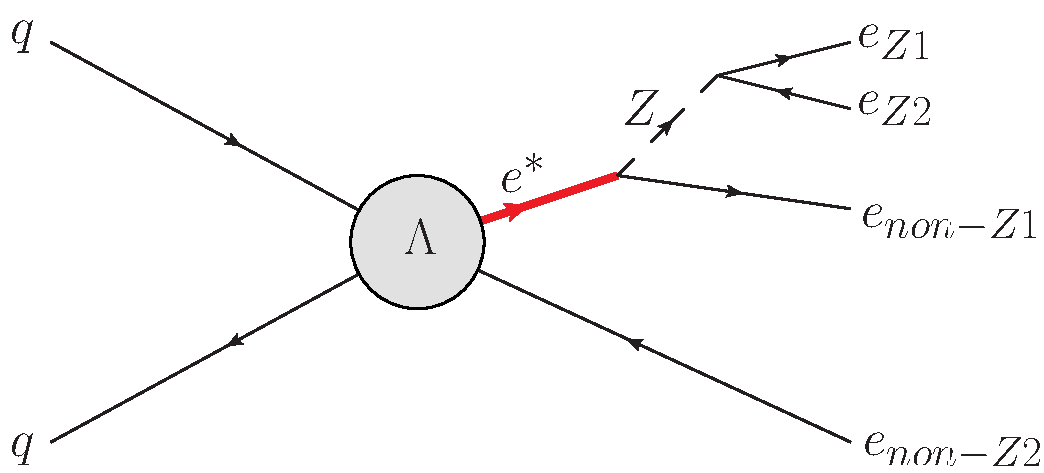
\includegraphics[width=0.49\textwidth]{plot/Feynman_Estar4e.pdf}  
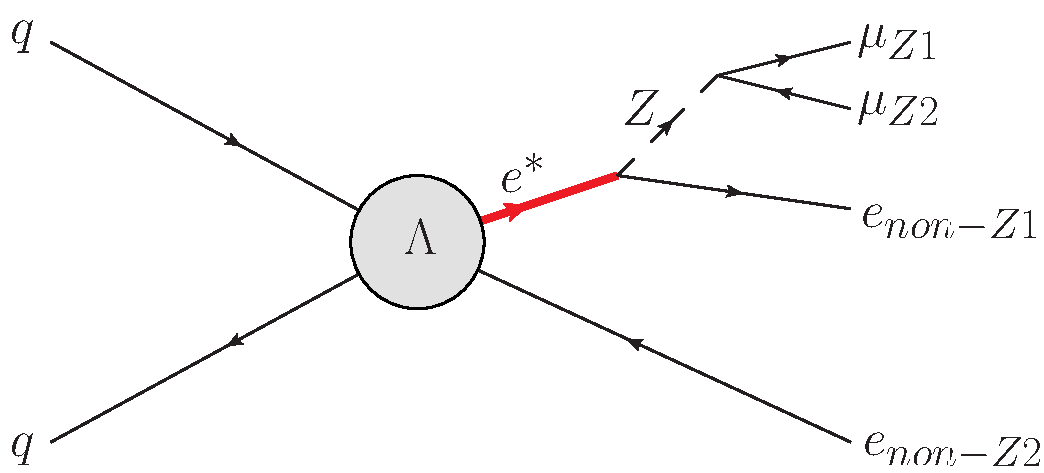
\includegraphics[width=0.49\textwidth]{plot/Feynman_Estar2e2mu.pdf}  
}
\caption{\label{fig:Feyman_ExLep}Feynman Diagrams for the investigated $l^{*}$ channels. (a) Excited muon. (b) Excited electron.}
\end{figure}
%%%%%%%%%%%%%%%%%%%%%%%%%%%%%%%%%%%%%%%%%%%%%%%%%%%%%%%%%%%%%%%%%%%%%%%%%%%%%%%%%%%%%%%%%%%%%%%%%%%%%%%%%%%%%%%%%%%%%%%%%%%%%%%%%%%%%%%%
\subsection{Decay of excited leptons}
Heavy excited leptons are expected to decay into SM leptons in a sudden they produced. The decay can occur via emitting a gauge bosons or four-fermion contact interaction. For the excited lepton mass greater than the vector bosons mass ($M_{l*} > M_{V}$), the partial widths of each gauge-mediated channels are shown in following equations.
\begin{align}
\Gamma (l^{*}\rightarrow lV) = \frac{1}{8}\frac{g_{V}^{2}}{4\pi}f_{V}^{2}\frac{M_{l*}^{3}}{\Lambda^{2}}\left\lgroup1 - \frac{M_{V}^{2}}{M_{l*}^{2}}\right\rgroup^{2}\left\lgroup2 + \frac{M_{V}^{2}}{M_{l*}^{2}}\right\rgroup
\end{align}
\noindent with
\begin{align}
f_{\gamma} = fT_{3} + f^{\prime}\frac{Y}{2}\\ 
f_{Z} = fT_{3}cos^{2}\theta_{W} - f^{\prime}\frac{Y}{2}sin^{2}\theta_{W}\\
f_{W} = \frac{f}{\sqrt{2}}
\end{align}

\noindent Here, $g_{V}$ denotes the corresponding coupling constants of each vector boson. For contact interaction, the width is obtained by
\begin{align}
\Gamma (l^{*}\rightarrow lf\bar{f}) = \frac{M_{l*}}{96\pi}\left\lgroup \frac{M_{l*}}{\Lambda}\right\rgroup^{4}N_{c}S^{\prime}
\end{align}
\noindent The $S^{\prime}$ is an additional combinatorical factor that $S^{\prime} = 2$ when $f = l$, and $S^{\prime} = 1$ otherwise. The $N_{c}$ represents the numbers of color. $N_{c} = 1(3)$ for $f$ represents a lepton(quark).
\newline From above equations, it can be seen that the branching ratio of each possible decay channel depands strongly on the value of coupling strength constants, $f$ and $f^{\prime}$), and the ratio of excited lepton mass over the compositeness scale($M_{l*}/\Lambda$). Fig. \ref{fig:BRff} shows the branching ratios of each decay mode of charged excited leptons with different $f / f^{\prime}$ values. The diffrent assumptions of $f$ and $f^{\prime}$ will result in different branching ratios among channels, and finally affect the limit setting. All gauge-mediated channels obtain a certain value of $f / f^{\prime}$ that the process is totally forbidden. For example, in the case of $f = -f^{\prime} = -1$, the photon-mediated channel gives out a partial width of zero. This give rises of the higher branching ratios of the Z-mediated channel, and can therefore reach a higher upper limit in this study than the case where $f = f^{\prime} = 1$ if no discovery claimed.     

\begin{figure}[h!]
\begin{center}
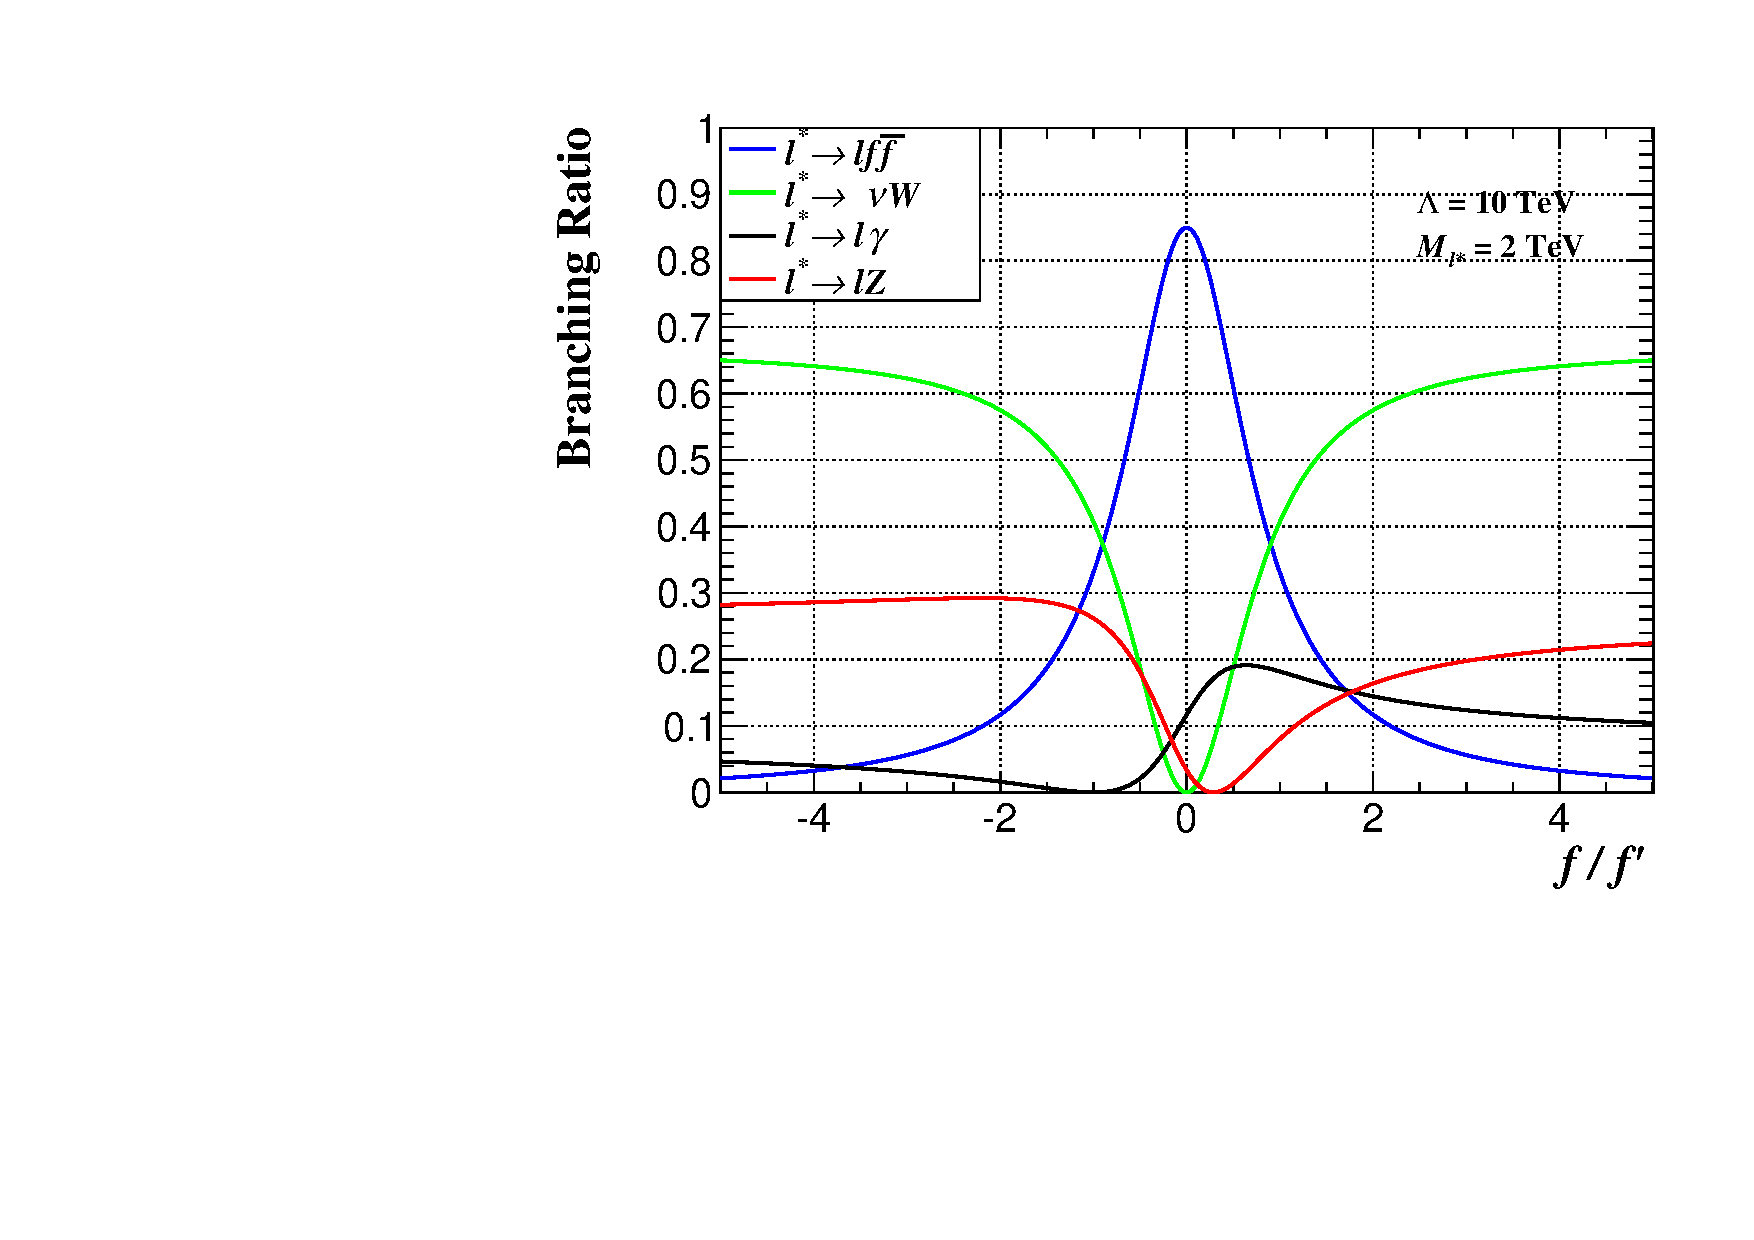
\includegraphics[width=0.9\textwidth]{plot/BRff.pdf}  
\caption{\label{fig:BRff}Branching ratios of charged excited leptons as function of $f / f^{\prime}$ with $\Lambda = 10 TeV$ and $M_{l*} = 2 TeV$.}
\end{center}
\end{figure}

Fig. \ref{fig:BR_ExLep} and Fig. \ref{fig:BR_ExLep_n1} shows the mass dependence of branching ratios with $f = f^{\prime}$ and $f = -f^{\prime}$ respectively for charged excited leptons. The cross-over structure for charged excited leptons with low mass is due to the square damping term in $f_{V}$. The decay via contact interaction becomes dominant as the $M_{l*}$ approches the $\Lambda$, due to the different dependence on $M_{l*} / \Lambda$ compare to gauge-mediated channels. For $M_{l*} = \Lambda$, the branching ratio of contact interaction reaches a value of 0.92, and only 0.08 for the sum of all gauge-mediated channels.  

\begin{figure}[h!]
\begin{center}
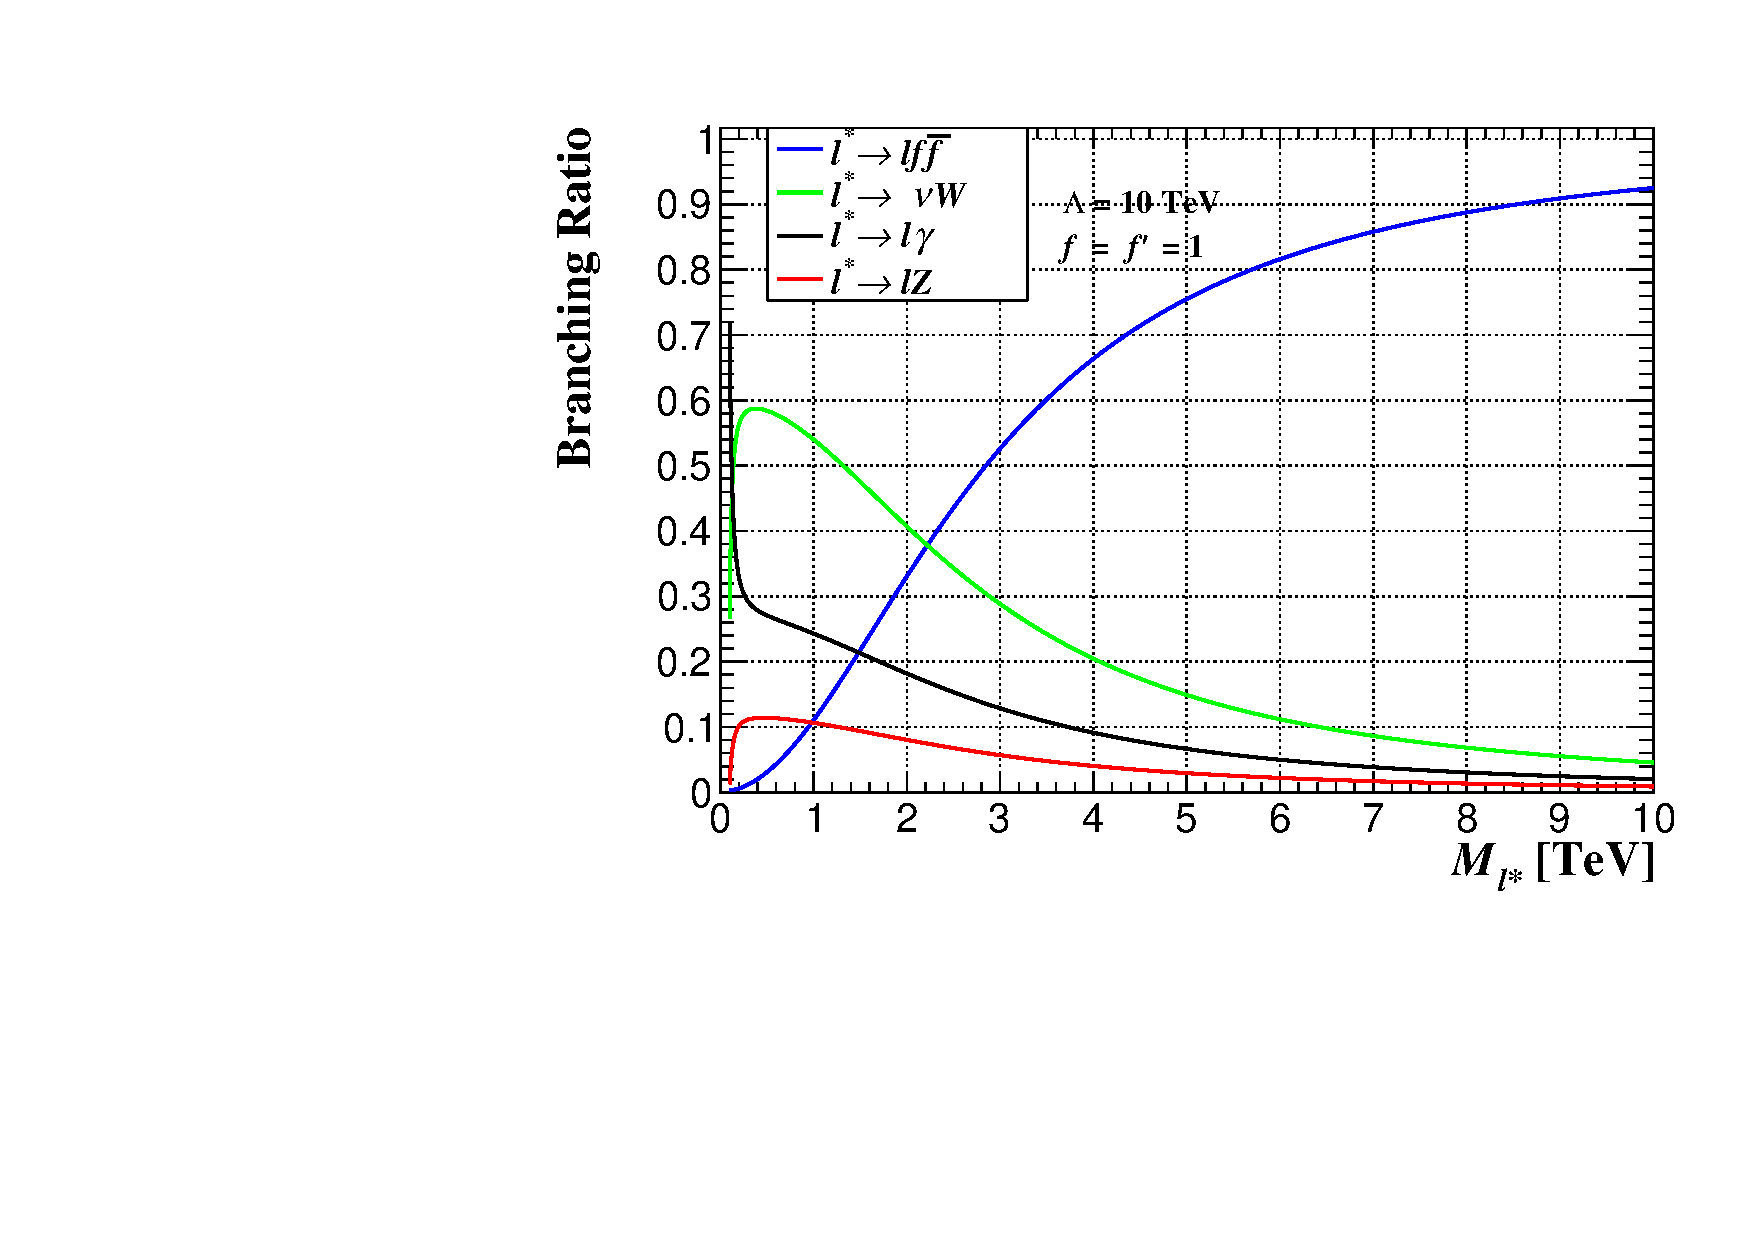
\includegraphics[width=0.9\textwidth]{plot/BR1.pdf}  
\caption{\label{fig:BR_ExLep}Branching ratios of charged excited leptons as function of $M_{l*}$ with $\Lambda = 10$ TeV and $f = f^{\prime} = 1$.}
\end{center}
\end{figure}

\begin{figure}[h!]
\begin{center}
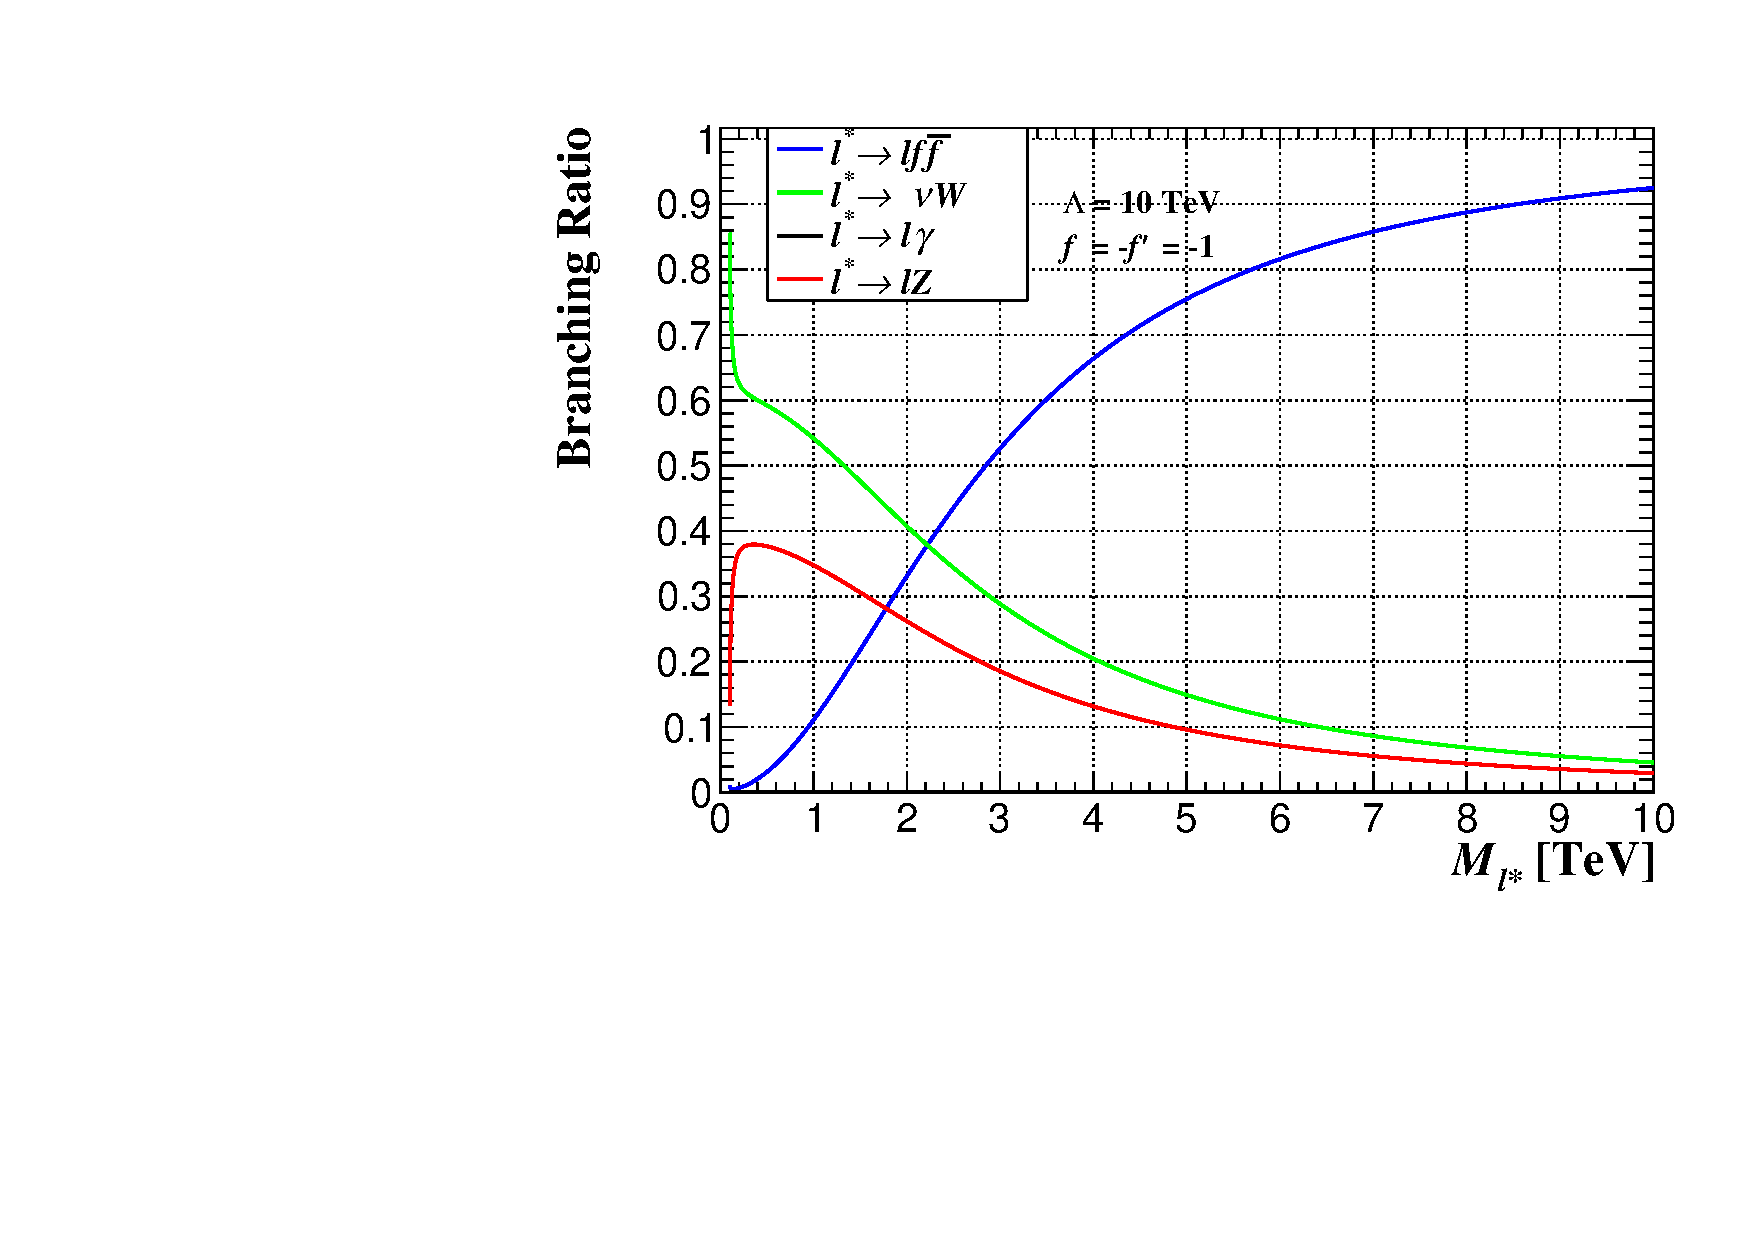
\includegraphics[width=0.9\textwidth]{plot/BRn1.pdf}  
\caption{\label{fig:BR_ExLep_n1}Branching ratios of charged excited leptons as function of $M_{l*}$ with $\Lambda = 10$ TeV and $f = -f^{\prime} = -1$.}
\end{center}
\end{figure}

\subsection{Production of excited leptons}
\label{sec:production}
Excited leptons can be produced singly or pairly through contact interactions in p-p collisions as shown in Fig. \ref{fig:ExLep_CI}. Base on the Lagrangian of the contact interaction, the cross section of excited lepton production can be obtained by

\begin{align}
\sigma_{single}(q\bar{q}\rightarrow l^{*}\bar{l}, l\bar{l}^{*}) = \frac{\pi}{6s} \left\lgroup \frac{s}{\Lambda^{2}}\right\rgroup^{2} \left\lgroup 1 + \frac{1}{3}\frac{s - M_{l*}^{2}}{s + M_{l*}^{2}}\right\rgroup \left\lgroup 1 - \frac{M_{l*}^{2}}{s} \right\rgroup^{2} \left\lgroup 1 + \frac{M_{l*}^{2}}{s} \right\rgroup 
\end{align}
\noindent and
\begin{align}
\sigma_{pair}(q\bar{q}\rightarrow l^{*}\bar{l}^{*}) = \frac{\pi}{9s}\left\lgroup 1 - 4\frac{M_{l*}^{2}}{s}\right\rgroup^{\frac{1}{2}} \left\lgroup \frac{s}{\Lambda^{2}}\right\rgroup^{2} \left\lgroup 1 - \frac{M_{l*}^{2}}{s}\right\rgroup
\end{align}

Fig. \ref{fig:XS} shows the cross section of the excited leptons single and pair production with $\Lambda = 10$ TeV. It can be seen that the cross section of single production is much larger than pair production. Moreover, the pair production will lead to rather complicate final states, and it is not too possible that a pair product events being removed with single production selection. Therefore, the normal strategy of the excited leptons search aims to search for single production events only.
\newline The cross section describe in this section is just a theoretical prediction of the excited leptons production. The actual used cross section in the experiments need further multiply a proper branching ratio depends on different final states and a leading order(LO) to next-to-leading order(NLO) correction factor. This cross section will be revealed in Sec. \ref{sec:Samples}.
\begin{figure}[h!]
\begin{center}
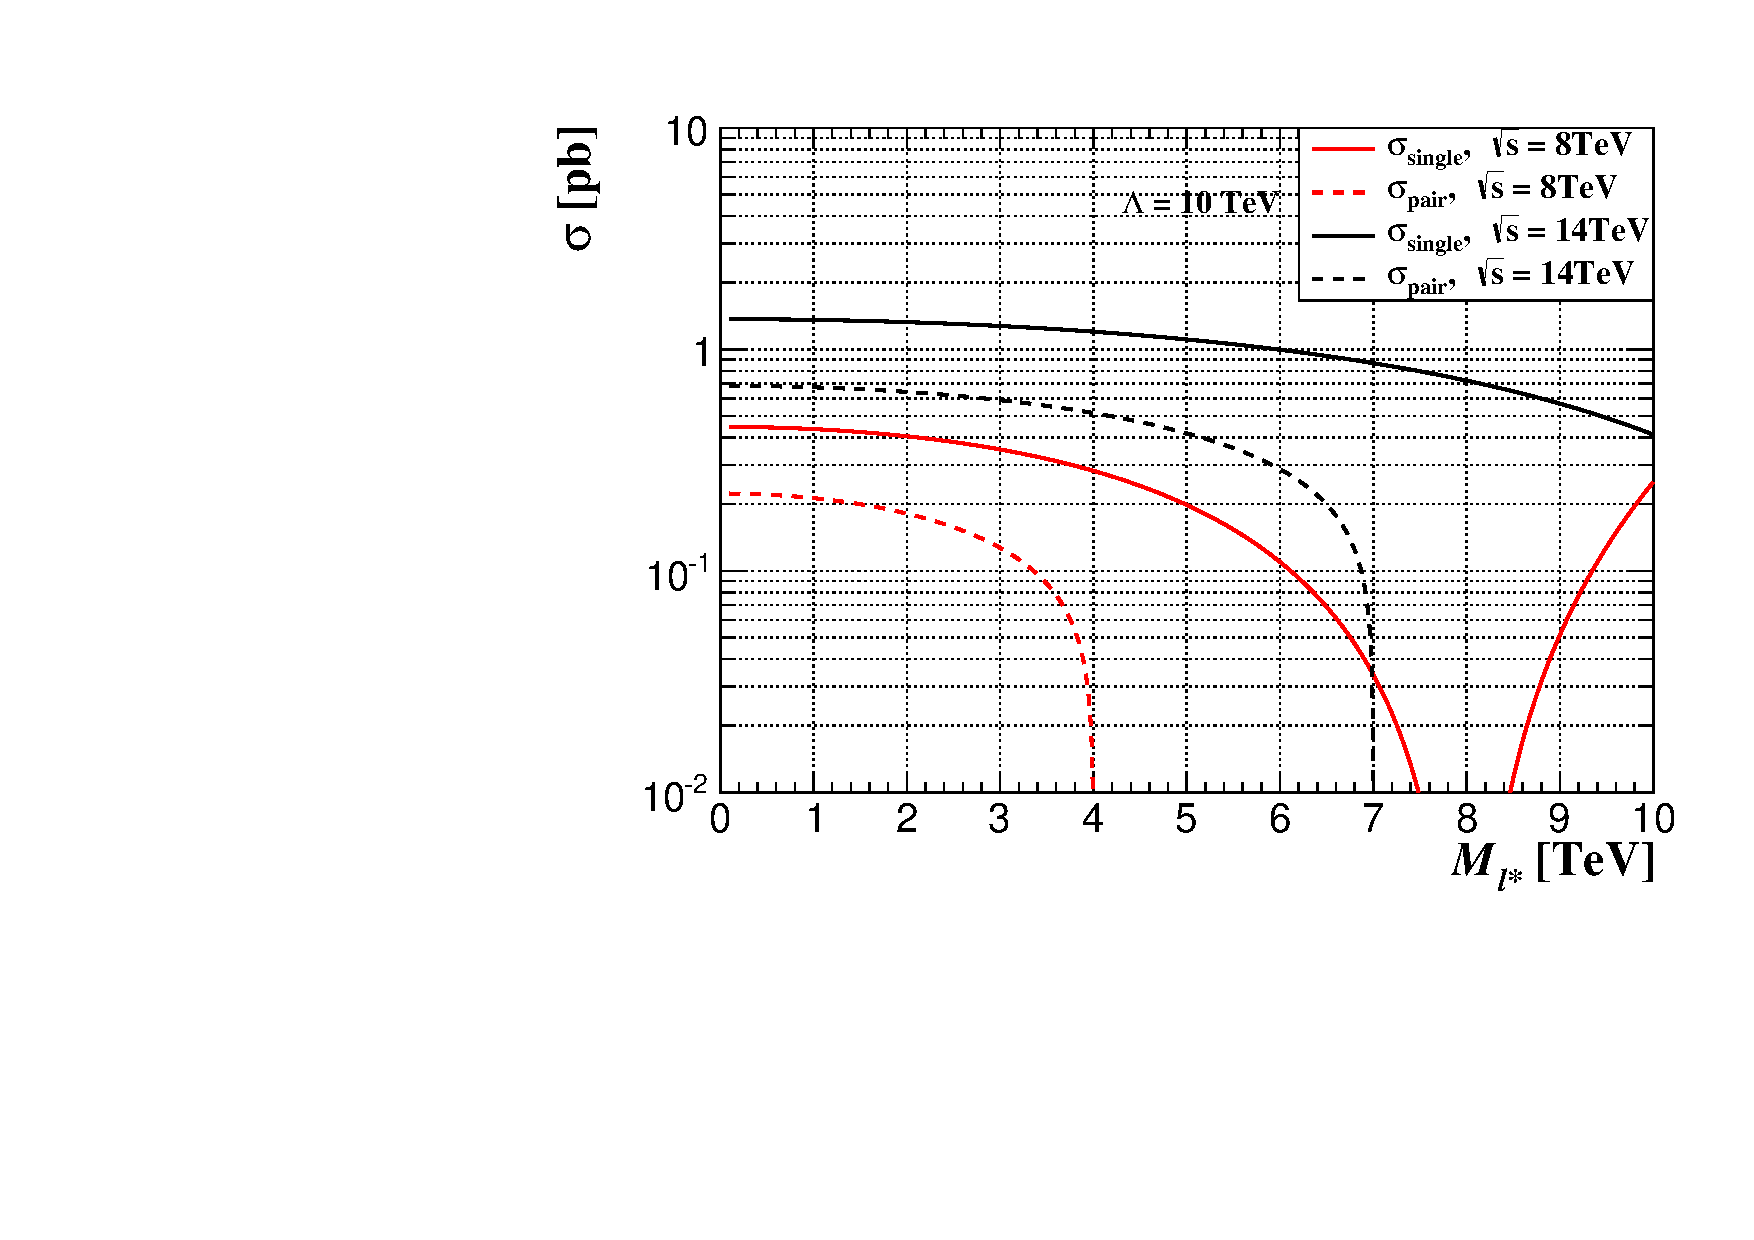
\includegraphics[width=0.9\textwidth]{plot/XS.pdf}  
\caption{\label{fig:XS}Cross section of charged excited leptons production as function of $M_{l*}$ with $\Lambda = 10$ TeV.}
\end{center}
\end{figure}
\newpage
